\section{Aplicativos}

Em uma busca realizada nas plataformas \emph{Play Store} e \emph{App Store},
para aplicativos móveis, e nas plataformas \emph{Steam} e \emph{Itch.io}, para
jogos digitais, foram identificados jogos correlatos. Utilizaram-se as
palavras-chave "Programação", "Estrutura de Dados" e "Jogo Educacional",
resultando inicialmente em um total de 262 jogos encontrados.

Após uma análise preliminar, 258 jogos foram descartados por não se enquadrarem
nos critérios da pesquisa. A maioria consistia em questionários ou aplicativos
de ensino que não se configuravam como jogos, enquanto outros apresentavam
temáticas não relacionadas à programação ou não atendiam aos requisitos mínimos
de qualidade. Com isso, restaram 4 jogos para a etapa de avaliação mais
detalhada.

\begin{enumerate}
  \subsection{Human Resource Machine}

Jogo de \emph{puzzle} desenvolvido pela \emph{Tomorrow Corporation}, tem como intuito ensinar lógica de programação de forma lúdica utilizando uma ambientação no meio corporativo, onde em cada fase o seu chefe lhe dá um trabalho e o seu objetivo é automatizar este trabalho programando pequenos trabalhadores para tal tarefa, e se você tiver sucesso nesta tarefa, será "promovido" para a próxima fase.
\cite{HumanResourceMachineSteam}

\begin{figure}[H]
	\centering
	\caption{Captura de tela do jogo Human Resource Machine}
	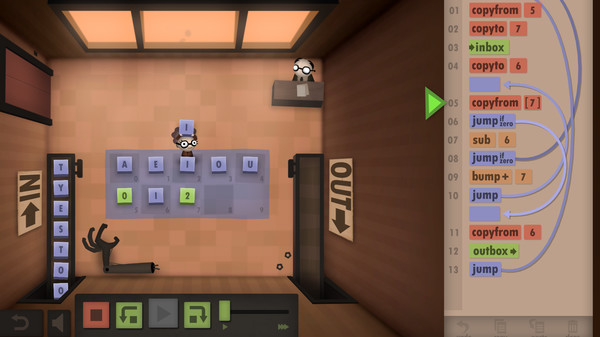
\includegraphics[width=0.8\textwidth]{images/human-resource-machine.jpg}
	\legend{Fonte: \cite{HumanResourceMachineSteam}}
	\label{fig:hrm}
\end{figure}


  \item \textbf{AlgoBot}

Jogo de \textit{puzzle} desenvolvido pela \textit{Fishing Cactus}, tem como
intuito ensinar algoritmos de forma lúdica utilizando uma ambientação
futuristica, onde o jogador tera o papel de operador que deverá criar uma
sequencia de commandos para o Algo Bot executar, seu objetivo é resolver
puzzles para terminar a sua missão de reciclagem. \cite{AlgoBotSteam}

\begin{figure}[H]
	\centering
	\caption{Captura de tela do jogo AlgoBot}
	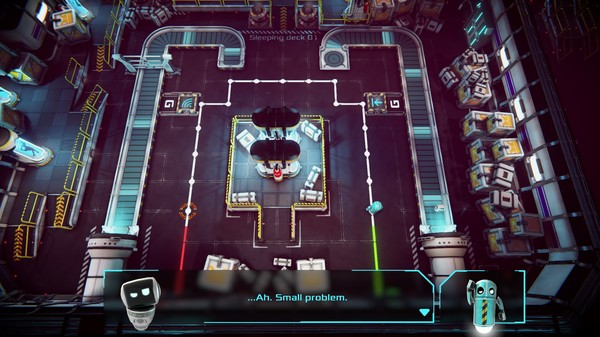
\includegraphics[width=0.8\textwidth]{images/algobot.jpg}
	\legend{Fonte: \cite{AlgoBotSteam}}
	\label{fig:ab}
\end{figure}


  \subsection{MOP'N SPARK}

Jogo de \textit{puzzle} desenvolvido pela \textit{Omoplata Games}, tem como intuito ensinar algoritmos de forma lúdica utilizando uma ambientação fantasiosa, onde o jogador deverá criar uma sequencia de commandos para que os personagens Bepp e Gola alcancem os seus objetivos. \cite{MOPNSPARKSteam}

\begin{figure}[H]
	\centering
	\caption{Captura de tela do jogo MOP'N SPARK}
	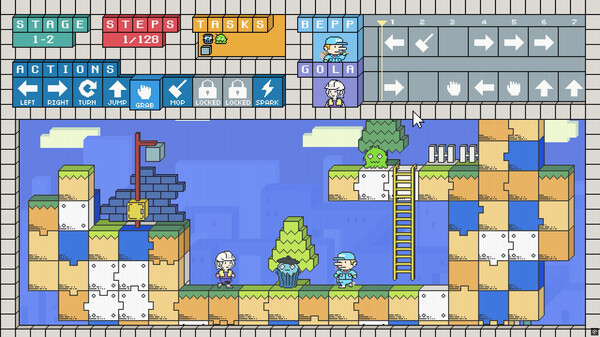
\includegraphics[width=0.8\textwidth]{images/mop-n-spark.jpg}
	\legend{Fonte: \cite{MOPNSPARKSteam}}
	\label{fig:mns}
\end{figure}


  \item \textbf{Iron Ears: Data Structure}

\textit{Iron Ears} é um jogo do gênero \textit{puzzle}, desenvolvido pela
\textit{NPC42 Games}, com o objetivo de ensinar conceitos de estruturas de
dados de forma interativa. Ambientado em um universo fictício habitado por
animais antropomorfizados, com inteligência e racionalidade comparáveis às
humanas.

O jogo coloca o jogador no papel de um coelho humanóide encarregado de
projetar e operar linhas de montagem de \textit{Mechs}. Esses robôs são
essenciais na resistência contra uma facção hostil que busca dominar o mundo.

A mecânica do jogo integra diretamente estruturas de dados clássicas, como
listas, filas e pilhas, aos sistemas de produção, exigindo que o jogador
aplique esses conceitos para resolver desafios e otimizar os processos de
fabricação. \cite{IronEarsItchio}

\begin{figure}[H]
	\centering
	\caption{Captura de tela do jogo Iron Ears}
	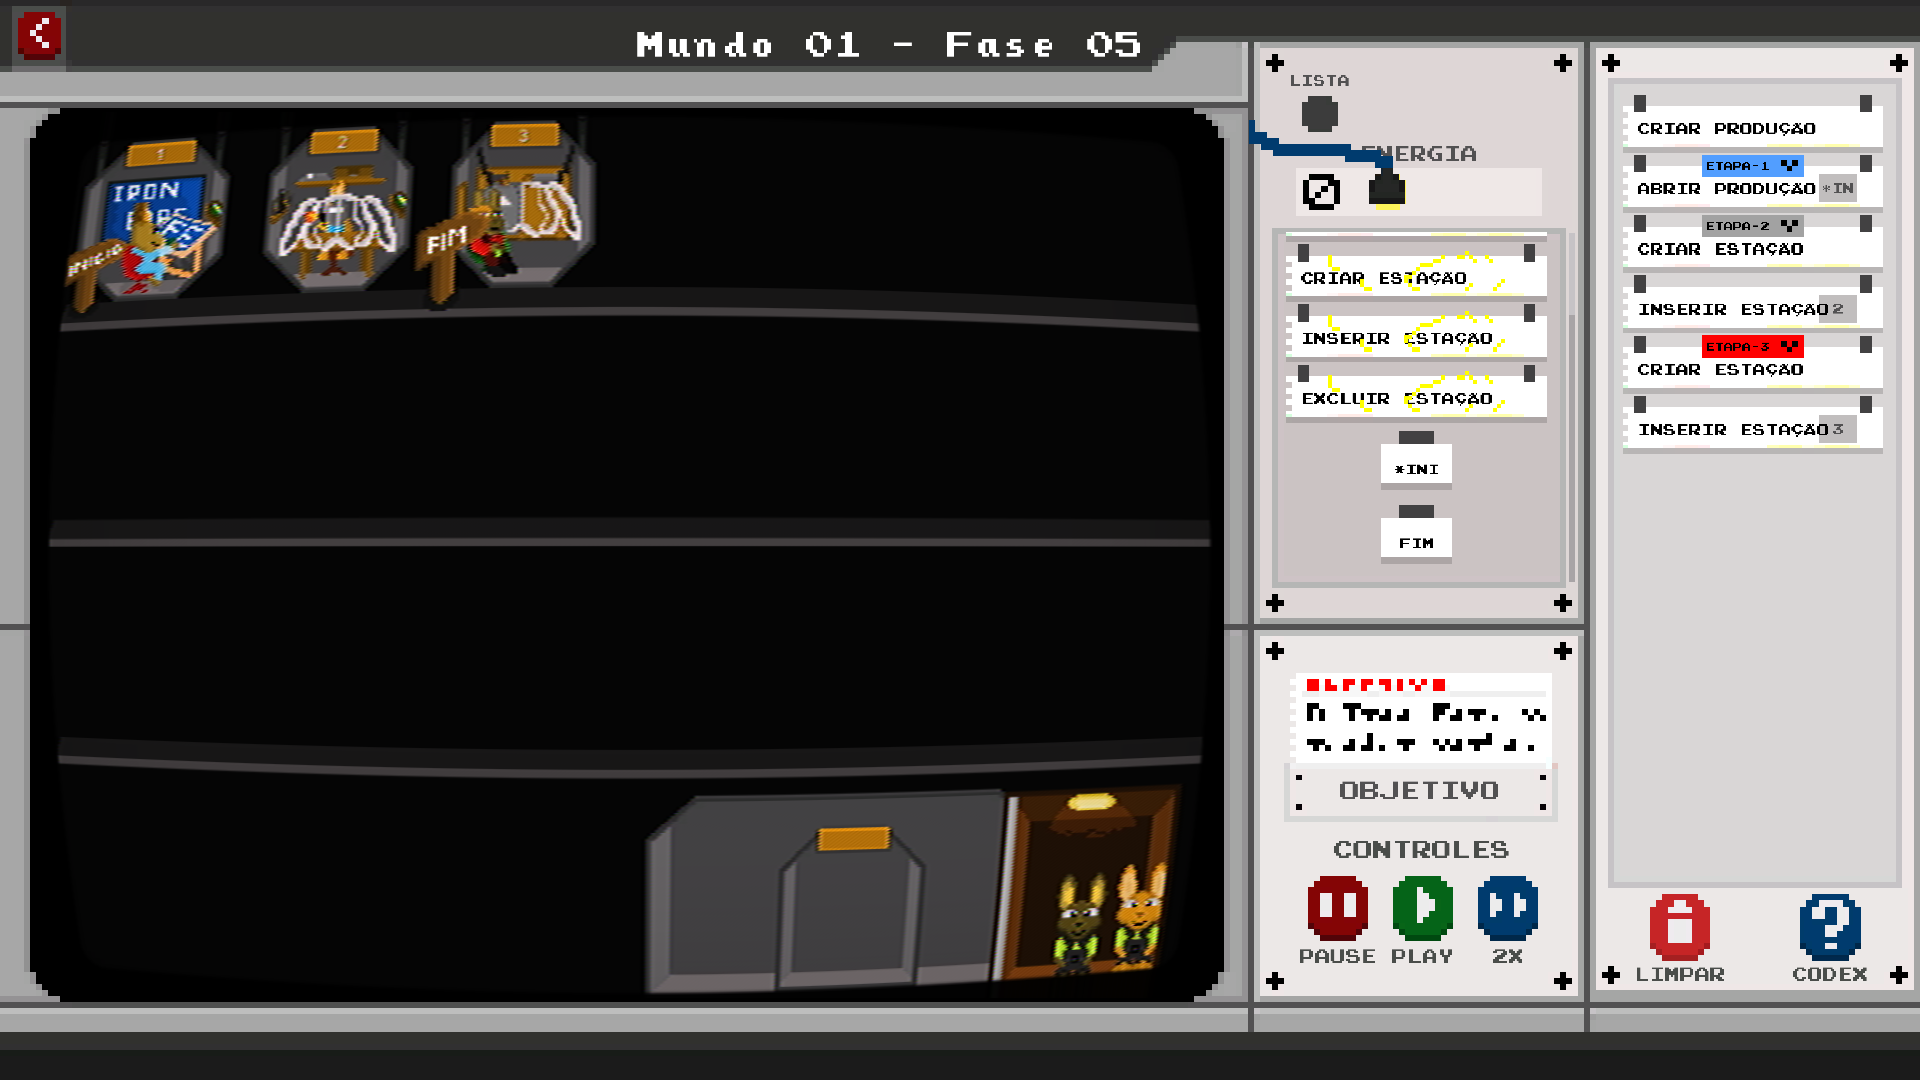
\includegraphics[width=0.8\textwidth]{images/iron-ears.png}
	\legend{Fonte: \cite{IronEarsItchio}}
	\label{fig:ie}
\end{figure}


\end{enumerate}

No tópico a seguir, é apresentada uma comparação entre os aplicativos selecionados.

\subsection{Comparação dos aplicativos}

A análise dos jogos selecionados revela uma variedade de abordagens no uso de
jogos sérios voltados ao ensino de lógica de programação. No entanto,
observa-se uma presença ainda limitada de propostas que exploram conceitos de
estruturas de dados de maneira mais aprofundada.

A \autoref{tab:cmp_jogos_relatos} apresenta uma síntese comparativa dessas
iniciativas, destacando os principais elementos de cada proposta. Os critérios
utilizados para esta comparação foram:

\begin{itemize}
  \item \textbf{Conceitos de Estrutura de Dados (CED)} - Quais conceitos foram abordados:
  \begin{itemize}
    \item Pilha (P)
    \item Fila (F)
    \item Lista (L)
  \end{itemize}
  \item \textbf{Forma de Abordagem Educacional (Ensino)} - Define se o ensino é tratado de forma explícita ou implícita.
  \item \textbf{Estilo} - Representação visual do jogo.
  \item \textbf{Gênero} - Categoria do jogo
  \item \textbf{Gratuito} - Indica se o jogo está disponível gratuitamente.
  \item \textbf{Avaliação} - Nota atribuída com base no sistema de avaliação da plataforma onde o jogo é disponibilizado.
\end{itemize}

Nos casos em que o jogo está disponível em plataformas que não possuem sistema
de avaliação integrado (como o \emph{itch.io}), ou em que não há avaliações
registradas, a avaliação é considerada \emph{indefinida}.

Para os jogos disponíveis na Steam, foi utilizada uma conversão aproximada
baseada na porcentagem de avaliações positivas, conforme mostrado na
\autoref{tab:avalicao_steam}.

\begin{table}[H]
	\caption{Comparação entre jogos relacionados e o trabalho proposto}
	\label{tab:cmp_jogos_relatos}
	\centering
	\footnotesize
	\begin{tabular}{r|clllll}
		\toprule
		\textbf{Trabalho}      & \textbf{ED}         & \textbf{Ensino}    & \textbf{Estilo}      & \textbf{Gênero}   & \textbf{Gratuito} & \textbf{Avaliação}  \\
		\midrule
		Human R.M.             & -                   & Explícito          & Top Down             & Puzzle            & Não               & 4.5                 \\
		AlgoBot                & -                   & Implícito          & Top Down             & Puzzle            & Não               & 4.2                 \\
		MOP'N SPARK            & -                   & Implícito          & Plataformer          & Puzzle            & Indefinido        & Indefinido          \\
		Iron Ears              & P,F,L               & Implícito          & Drag \& Drop         & Puzzle            & Sim               & Indefinido          \\
		\rowcolor{gray!20}
		\textbf{Este trabalho} & \textbf{P,F,LE,B,O} & \textbf{Implícito} & \textbf{Plataformer} & \textbf{Aventura} & \textbf{Sim}      & \textbf{Indefinido} \\
		\bottomrule
	\end{tabular}

	\vspace{1.25em}
	\begin{minipage}{0.8\linewidth}
		\footnotesize
		\textbf{CED:} Conceitos de Estrutura de Dados utilizados -
		\textbf{P:} Pilha, \textbf{F:} Fila, \textbf{L:} Lista, \textbf{LE:} Lista Encadeada, \textbf{B:} Algoritmo de Busca, \textbf{O:} Algoritmo de Ordenação. \\
		\textbf{Ensino:} Forma de abordagem educacional (Explícito ou Implícito). \\
		\textbf{Estilo:} Estilo de interação do jogo. - \textbf{P\&C:} Point and Click \\
		\textbf{Gênero:} Categoria do jogo. \\
		\textbf{Gratuito:} Se o jogo é gratuito ou não. \\
		\textbf{Avaliação:} Avaliação do jogo, \textbf{indefinido} ocorre quando a plataform que disponibiliza o jogo não possui um sistema de avaliação, como o itch.io, ou nenhuma avaliação foi feita ao jogo. Jogos da steam possuem um sistema de avaliação próprio e por conta disto foi feito uma conversão aproximada apresentada na \autoref{tab:avalicao_steam}
	\end{minipage}
\end{table}


\begin{table}[H]
	\caption{Conversão do Sistema de Avaliação da Steam para um sistema numeral de 1 a 5}
	\label{tab:avalicao_steam}
	\centering
	\footnotesize
	\begin{tabular}{clc}
		\toprule
		\textbf{Porcentagem de Avaliações Positivas} & \textbf{Avaliação Steam} & \textbf{Conversão Aproximada} \\
		\midrule
		90\% - 100\%                                 & Extremamente positivas   & 4.5 - 5.0                     \\
		70\% - 89\%                                  & Muito positivas          & 3.5 - 4.4                     \\
		40\% - 69\%                                  & Neutras                  & 2.0 - 3.4                     \\
		10\% - 39\%                                  & Muito Negativas          & 0.5 - 1.9                     \\
		0\% -  9\%                                   & Extremamente negativas   & 0.0 - 0.4                     \\
		\bottomrule
	\end{tabular}
	\caption*{Fonte: Autor}
\end{table}


O cálculo utilizado para a conversão é dado pela fórmula:

\[
  \text{Porcentagem de Avaliações Positivas} \times \frac{5}{100}
\]

